% @Author: AnthonyKenny98
% @Date:   2020-04-05 12:55:29
% @Last Modified by:   AnthonyKenny98
% @Last Modified time: 2020-04-05 15:43:13

\begin{figure}[H]
\begin{centering}

\begin{tabular}{cc}
\begin{subfigure}{0.45\linewidth}
    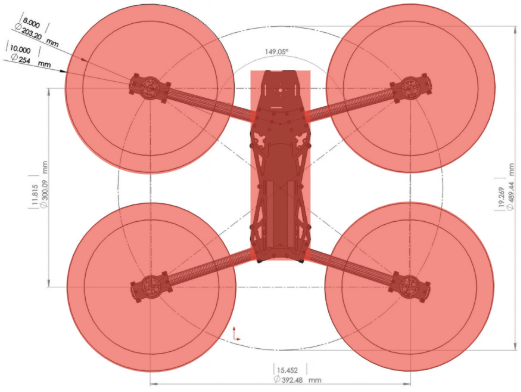
\includegraphics[width=\linewidth]{appendices/rrt/img/DroneNegSpace.png}
    \caption{}
    \label{subfig:dronenegspace}
\end{subfigure}
\begin{subfigure}{0.45\linewidth}
    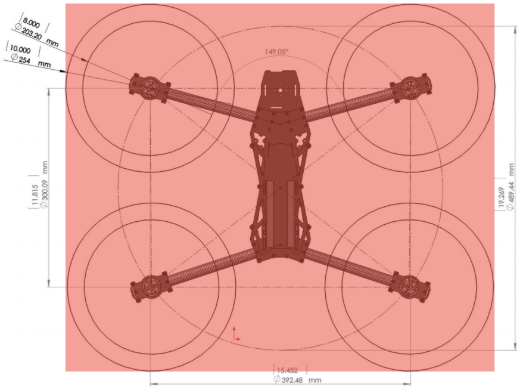
\includegraphics[width=\linewidth]{appendices/rrt/img/DroneRecPrism.png}
    \caption{}
    \label{subfig:dronerecprism}
\end{subfigure}
\end{tabular}
\caption[Modelling a UAV as a Rectangular Prism]{Modelling a \gls{UAV} as a Rectangular Prism. Red highlight demonstrates the model, overlayed over the exact schematic. Figure \ref{subfig:dronenegspace} shows how a drone can be modelled in high detail, but gains little useful free space when compared with Figure \ref{subfig:dronerecprism}, which models a drone as a rectangular prism.\cite{Thingbits}}
\label{fig:dronemodelling}
\end{centering}
\end{figure}